\documentclass[]{article}
\usepackage{geometry,tikz,lipsum,amsmath,amssymb,mathrsfs,soul,xcolor,cancel,esint,graphicx}
\tikzset{every picture/.style={line width=0.75pt}} %set default line width to 0.75pt        
\numberwithin{equation}{section}

\NewDocumentCommand{\caja}{ m O{gray!40} O{gray!10} m }{
	\begin{figure}[h]
		\centering
		\begin{tikzpicture}
			\node[anchor=text, text width=\columnwidth-1.2cm, draw, rounded corners, line width=1pt, fill=#3, inner sep=5mm] (big) {\\#4};
			\node[draw, rounded corners, line width=.5pt, fill=#2, anchor=west, xshift=5mm] (small) at (big.north west) {#1};
		\end{tikzpicture}
	\end{figure}
}

\newcommand{\deriv}[3]{\left(\frac{\partial #1}{\partial #2} \right)_{#3}}

\newcommand{\dderiv}[3]{\left(\dfrac{\partial #1}{\partial #2} \right)_{#3}}

\NewDocumentCommand{\indUpDown}{ O{\Lambda} O{\mu} O{\nu} }{
{#1}^{#2}_{\ #3}
}
\NewDocumentCommand{\indDownUp}{ O{\Lambda} O{\mu} O{\nu} }{
{#1}_{#2}^{\ #3}
}

\newcommand{\LambdaMuNu}{\indUpDown}
\newcommand{\0}{\textcolor{gray}{0}}
\newcommand{\ei}{\mathbf{e}_i}
\newcommand{\ej}{\mathbf{e}_j}
\newcommand{\lc}{\epsilon_{ijk}}
\newcommand{\gr}{\nabla}
\newcommand{\di}{\nabla\cdot}
\newcommand{\ro}{\nabla\times}
\newcommand{\la}{\nabla^2}
\newcommand{\rv}{\mathbf{r}}
\newcommand{\pv}{\mathbf{p}}
\newcommand{\xv}{\mathbf{x}}
\newcommand{\yv}{\mathbf{y}}
\newcommand{\zv}{\mathbf{z}}
\newcommand{\xhat}{\hat{\xv}}
\newcommand{\yhat}{\hat{\yv}}
\newcommand{\zhat}{\hat{\zv}}
\newcommand{\ihat}{\hat{\mathbf{i}}}
\newcommand{\jhat}{\hat{\mathbf{j}}}
\newcommand{\khat}{\hat{\mathbf{k}}}
\newcommand{\rhat}{\hat{\rv}}
\newcommand{\that}{\hat{\mathbf{\theta}}}
\newcommand{\phat}{\hat{\mathbf{\varphi}}}
\newcommand{\rhhat}{\hat{\mathbf{\rho}}}
\newcommand{\nhat}{\hat{\mathbf{n}}}
\newcommand{\Rhat}{\hat{\mathbf{R}}}
\newcommand{\eo}{\epsilon_{0}}
\newcommand{\uo}{\mu_{0}}
\NewDocumentCommand{\ke}{ O{1}}{
\frac{#1}{4\pi\eo}
}
\NewDocumentCommand{\ku}{ O{}}{
\frac{\uo #1}{4\pi}
}
%\newcommand{\ke}{\frac{1}{4\pi\eo}}
%\newcommand{\ku}{\frac{\uo}{4\pi}}
\newcommand{\rdif}{\rv - \rv'}
\newcommand{\pd}[2]{\dfrac{\partial #1}{\partial #2}}
\newcommand{\lpd}[2]{\partial #1/\partial #2}
\newcommand{\spd}[2]{\frac{\partial #1}{\partial #2}}
\newcommand{\td}[2]{\dfrac{d #1}{d #2}}
\newcommand{\ltd}[2]{d #1/d #2}
\newcommand{\std}[2]{\frac{d #1}{d #2}}
\newcommand{\n}[1]{\mathbf{#1}}
\newcommand{\eff}[1]{#1_\mathrm{eff}}
\newcommand{\Ueff}{\eff{U}}

\newcommand{\wfrac}[3][3pt]{%
\frac{\wfracterm{depth}{\dp}{#1}{#2}}{\wfracterm{height}{\ht}{#1}{#3}}%
}
\newcommand{\wfracterm}[4]{%
\sbox0{$\displaystyle#4$}%
\vrule width 0pt #1 \dimexpr #20+#3\relax
\usebox{0}%
}

\newcommand{\pr}[1]{\left\langle #1 \right\rangle }

\newcommand{\qed}{\hfill\(\blacksquare\)}
\newcommand{\resp}{
	\\
	
	\textbf{Respuesta:} }
\newcommand{\celsius}{^\circ\mathrm{C}}

%opening
\title{Tarea 2 Mecánica Estadística Avanzada}
\author{Simon Fonseca}

\begin{document}
\maketitle

Como segunda tarea corresponde a realizar 8 de los 17 problemas 4-7, 4-8, 4-13, 4-14, 4-15, 4-21 (capítulo 4), 6-1, 6-23, 6-24, 6-25, 6-26 (capítulo 6), 8-15, 8-16 (capítulo 8), 9-1, 9-2, 9-4, 9-8 (capítulo 9) del libro de Mc. Quarrie

%%%%%%%%%%%%%%%%%%%%%%%%%%%%%%%%%%%%%%%%%%%%%%%%%%%%%%%%%%%%%%%%%%%%%%%%%%%%%%%%%%%%%%%%%%%%%%%%%%%%%%%%
\section{Problema 4.7}
Recall that the equation of state for an ideal quantum gas is
\begin{equation}
	pV = kT\ln\Xi = \pm kT \sum_{j}\ln\left[1 \pm \lambda e^{-\epsilon_j/kT}\right]
\end{equation}
where $\lambda = e^{\mu/kT}$. Using the fact that the summation over states can be replaced by an integration over energy levels
\begin{equation}
	\omega(\epsilon) \, d\epsilon = 2\pi \left(\frac{2m}{h^2}\right)^{3/2} V \sqrt{\epsilon} \, d\epsilon
\end{equation}
derive the quantum virial expansion
\begin{equation}
	\frac{p}{kT} = \mp \frac{1}{\Lambda^3} \sum_{j=1}^{\infty} \frac{(\mp 1)^j \lambda^j}{j^{5/2}}
\end{equation}
where $\Lambda = \sqrt{h^2 / 2\pi m k T}$.
\resp Partiendo de la ecuación de estado y pasando a una integral
\begin{align*}
	pV &= \pm kT \sum_{j}\ln\left[1 \pm \lambda e^{-\epsilon_j/kT}\right]\\
	&= \pm kT \int_{0}^{\infty} \ln\left[1 \pm \lambda e^{-\epsilon_j/kT}\right] \omega(\epsilon) \, d\epsilon\\
	&= \pm kT \int_{0}^{\infty} \ln\left[1 \pm \lambda e^{-\epsilon_j/kT}\right] \cdot 2\pi \left(\frac{2m}{h^2}\right)^{3/2} V \sqrt{\epsilon} \, d\epsilon\\
	\Rightarrow \frac{p}{kT} &= \pm 2\pi \left(\frac{2m}{h^2}\right)^{3/2} \int_{0}^{\infty} \ln\left[1 \pm \lambda e^{-\epsilon_j/kT}\right] \sqrt{\epsilon} \, d\epsilon
\end{align*}
Podemos expandir el logaritmo usando series de Taylor y obtener
\begin{equation*}
	\ln\left[1 + x\right] = \sum_{j=1}^{\infty} \frac{(-1)^{j+1}}{j} \, x^j
\end{equation*}
Reemplazando $x = \pm \lambda e^{-\epsilon_j/kT}$
\begin{equation*}
	\ln\left[1 \pm \lambda e^{-\epsilon_j/kT}\right] = \sum_{j=1}^{\infty} \frac{(-1)^{j+1}}{j} \, (\pm)^j \lambda^{j} e^{-j \epsilon_j/kT} = \sum_{j=1}^{\infty} \frac{(\mp 1)^{j+1}}{j} \lambda^{j} e^{-j \epsilon_j/kT}
\end{equation*}
Por lo que
\begin{align}
	\frac{p}{kT} &= \pm 2\pi \left(\frac{2m}{h^2}\right)^{3/2} \int_{0}^{\infty} \sum_{j=1}^{\infty} \frac{(\mp 1)^{j+1}}{j} \lambda^{j} e^{-j \epsilon_j/kT} \sqrt{\epsilon} \, d\epsilon \nonumber\\
	&= \pm 2\pi \left(\frac{2m}{h^2}\right)^{3/2} \sum_{j=1}^{\infty} \frac{(\mp 1)^{j+1}}{j} \lambda^{j} \int_{0}^{\infty} e^{-j \epsilon_j/kT} \sqrt{\epsilon} \, d\epsilon \nonumber\\
	&= \pm 2\pi \left(\frac{2m}{h^2}\right)^{3/2} \sum_{j=1}^{\infty} \frac{(\mp 1)^{j+1}}{j} \lambda^{j} \cdot \frac{\sqrt{\pi }}{2 \left(\frac{j}{k T}\right)^{3/2}} \nonumber\\
	&= \pm \frac{2\pi \sqrt{\pi} \left(k T\right)^{3/2}}{2} \left(\frac{2m}{h^2}\right)^{3/2} \sum_{j=1}^{\infty} \frac{(\mp 1)^{j+1}}{j} \frac{\lambda^{j}}{j^{3/2}} \nonumber\\
	&= \pm \left(\frac{2 \pi k T m}{h^2}\right)^{3/2} \sum_{j=1}^{\infty} \frac{(\mp 1)^{j+1} \lambda^{j}}{j^{5/2}} \nonumber
	\intertext{Usando $\Lambda = \sqrt{h^2 / 2\pi m k T}$,}
	&= \pm \frac{1}{\Lambda^3} \sum_{j=1}^{\infty} \frac{\mp 1 \cdot (\mp 1)^{j} \lambda^{j}}{j^{5/2}} \nonumber\\
	\frac{p}{kT} &= \mp \frac{1}{\Lambda^3} \sum_{j=1}^{\infty} \frac{(\mp 1)^{j} \lambda^{j}}{j^{5/2}}
\end{align}
\qed

%%%%%%%%%%%%%%%%%%%%%%%%%%%%%%%%%%%%%%%%%%%%%%%%%%%%%%%%%%%%%%%%%%%%%%%%%%%%%%%%%%%%%%%%%%%%%%%%%%%%%%%%
\section{Problema 4.8}
Show that the entropy of an ideal quantum gas can be written as
\begin{equation}
	S = - k \sum_{j} \left[\bar{n}_j \ln \bar{n}_j \pm \left(1 \mp \bar{n}_j\right)\ln\left(1 \mp \bar{n}_j\right)\right]
\end{equation}
where the upper (lower) sign denotes Fermi-Dirac (Bose-Einstein) statistics.
\resp 
Tenemos la relación
\begin{align}
	TS &= \pr{E} - \mu\pr{N} - \Omega \nonumber\\
	\Rightarrow S &= \frac{1}{T}\pr{E} - \frac{1}{T}\mu\pr{N} - \frac{1}{T}\Omega
\end{align}
donde $\Omega$ es el potencial gran canónico
\begin{equation*}
	\Omega = - k T \ln \Xi
\end{equation*}
Utilizando la ecuación de estado obtendremos
\begin{align*}
	\Omega &= - k T \cdot \pm \sum_{j}\ln \left[1 \pm \lambda e^{-\epsilon_j/kT}\right]\\
	&= \mp k T \sum_{j}\ln \left[1 \pm \lambda e^{-\epsilon_j/kT}\right]
\end{align*}
donde $\lambda = e^{\mu/kT}$. Por otro lado, el número promedio de partículas en el $j$-ésimo estado cuántico es
\begin{equation}
	\bar{n}_j = \frac{\lambda e^{-\epsilon_j/kT}}{1 \pm \lambda e^{-\epsilon_j/kT}}
\end{equation}
Si intentamos aislar el término $\lambda e^{-\epsilon_j/kT}$ (que también aparece en la ec. de estado), obtendremos
\begin{align*}
	\bar{n}_j &= \lambda e^{-\epsilon_j/kT} \cdot \frac{1}{1 \pm \lambda e^{-\epsilon_j/kT}}\\
	\Rightarrow \lambda e^{-\epsilon_j/kT} &= \left(1 \pm \lambda e^{-\epsilon_j/kT}\right) \cdot \bar{n}_j\\
	\lambda e^{-\epsilon_j/kT} &= \bar{n}_j \pm \lambda e^{-\epsilon_j/kT} \cdot \bar{n}_j \\
	\lambda e^{-\epsilon_j/kT} \mp \lambda e^{-\epsilon_j/kT} \cdot \bar{n}_j &= \bar{n}_j \\
	\lambda e^{-\epsilon_j/kT} \left( 1 \mp \bar{n}_j\right) &= \bar{n}_j \\
	\Rightarrow \lambda e^{-\epsilon_j/kT} &= \frac{\bar{n}_j}{\left( 1 \mp \bar{n}_j\right)}
\end{align*}
Reemplazando en la ec. de estado,
\begin{align}
	\Omega &= \mp k T \sum_{j}\ln \left[1 \pm \frac{\bar{n}_j}{\left( 1 \mp \bar{n}_j\right)}\right] \nonumber\\
	&= \mp k T \sum_{j}\ln \left[\frac{ 1 \mp \bar{n}_j \pm \bar{n}_j}{\left( 1 \mp \bar{n}_j\right)}\right] \nonumber\\
	&= \mp k T \sum_{j}\ln \left[\frac{ 1 }{\left( 1 \mp \bar{n}_j\right)}\right] \nonumber\\
	\Omega = - k T \ln \Xi &= \pm k T \sum_{j}\ln \left[1 \mp \bar{n}_j \right]\\
	\ln \Xi &= \mp \sum_{j}\ln \left[1 \mp \bar{n}_j \right]
\end{align}
Luego, para los valores de $\pr{E}$ y $\pr{N}$, podemos usar las definiciones
\begin{equation}
	\pr{E} = \sum_{j} \epsilon_j \bar{n}_j, ~~~~~ \pr{N} = \sum_{j} \bar{n}_j, ~~~~~ \mu = kT \ln\lambda
\end{equation}
Reemplazando en la relación original,
\begin{align*}
	S &= \frac{1}{T}\sum_{j} \epsilon_j \bar{n}_j - \frac{1}{T}kT \ln\lambda\sum_{j} \bar{n}_j \mp \frac{1}{T}\cdot k T \sum_{j} \ln \left[1 \mp \bar{n}_j \right] \\
	&= \sum_{j} \frac{\epsilon_j \bar{n}_j}{T} - k  \bar{n}_j \ln\lambda \mp k \ln \left[1 \mp \bar{n}_j \right]
\end{align*}
pero
\begin{align*}
	\ln\lambda &= \ln \left[e^{\epsilon_j/kT} \frac{\bar{n}_j}{\left( 1 \mp \bar{n}_j\right)}\right]\\
	&= \frac{\epsilon_j}{kT} + \ln\left[\frac{\bar{n}_j}{\left( 1 \mp \bar{n}_j\right)}\right]
\end{align*}
por lo que
\begin{align*}
	S &= \sum_{j} \frac{\epsilon_j \bar{n}_j}{T} - k  \bar{n}_j\left( \frac{\epsilon_j}{kT} + \ln\left[\frac{\bar{n}_j}{\left( 1 \mp \bar{n}_j\right)}\right]\right) \mp k \ln \left[1 \mp \bar{n}_j \right]\\
	&= \sum_{j} \frac{\epsilon_j \bar{n}_j}{T} - \frac{\epsilon_j \bar{n}_j}{T} - k  \bar{n}_j \ln\left[\frac{\bar{n}_j}{\left( 1 \mp \bar{n}_j\right)}\right] \mp k \ln \left[1 \mp \bar{n}_j \right]\\
	&= k\sum_{j} - \bar{n}_j \ln\bar{n}_j + \bar{n}_j \ln \left[ 1 \mp \bar{n}_j\right] \mp \ln \left[1 \mp \bar{n}_j \right]\\
	&= k\sum_{j} (\bar{n}_j \mp 1) \ln \left[1 \mp \bar{n}_j \right] - \bar{n}_j \ln\bar{n}_j \\
	&= -k\sum_{j} \bar{n}_j \ln\bar{n}_j - (\bar{n}_j \mp 1) \ln \left[1 \mp \bar{n}_j \right] \\
	&= -k\sum_{j} \bar{n}_j \ln\bar{n}_j \pm (1 \mp \bar{n}_j) \ln \left[1 \mp \bar{n}_j \right]
\end{align*}
\qed

%%%%%%%%%%%%%%%%%%%%%%%%%%%%%%%%%%%%%%%%%%%%%%%%%%%%%%%%%%%%%%%%%%%%%%%%%%%%%%%%%%%%%%%%%%%%%%%%%%%%%%%%
\section{Problema 4.13}
The vibrational energy levels of a diatomic molecule can be approximated by a quantum mechanical harmonic oscillator. The fundamental vibrational frequency $\nu$ is $O(10^{13} \, \mathrm{[sec^{-1}]})$ for many diatomic molecules. Calculate the fraction of molecules in the first few vibrational levels in an ideal diatomic gas at $25^\circ\mathrm{C}$. Derive a closed expression for the fraction of molecules in all excited states.
\resp La fracción de moléculas en un nivel energético $j$ vendrá dado por
\begin{equation}
	\pi_j = \frac{e^{-\epsilon_j/kT}}{Z}
\end{equation}
donde $Z$ es la función de partición. Considerando los niveles de energía de un oscilador armónico cuántico:
\begin{equation}
	\epsilon_j = \left(j + \frac{1}{2}\right) h \nu
\end{equation}
Luego, con la ecuación de partición canónica y reemplazando la energía
\begin{equation*}
	Z = \sum_{j=0}^{\infty} e^{-\epsilon_j/kT} = e^{-h\nu/2kT} \sum_{j=0}^{\infty} e^{-j h \nu/kT}
\end{equation*}
Usando el resultado de la serie geométrica $\sum_{j=0}^{\infty} a r^j = a/(1-r)$, donde $a = 1, ~ r = e^{-h\nu/kT}$, tenemos
\begin{equation*}
	Z = \frac{e^{-h\nu/2kT}}{1 - e^{-h\nu/kT}}
\end{equation*}
Volviendo a la fracción de partículas según nivel de energía,
\begin{align}
	\pi_j &= \frac{e^{-\epsilon_j/kT}}{Z} \nonumber\\
	&= \frac{e^{-\left(j + 1/2\right) h \nu/kT} \left(1 - e^{-h\nu/kT}\right)}{e^{-h\nu/2kT}}\nonumber\\
	&= \frac{e^{-j h \nu/kT} e^{-h \nu/2kT} \left(1 - e^{-h\nu/kT}\right)}{e^{-h\nu/2kT}}\nonumber\\
	&= e^{-j h \nu/kT} \left(1 - e^{-h\nu/kT}\right)
\end{align}
Tomando
\begin{equation*}
	h \approx 6.626 \times 10^{-34} \, \mathrm{[J \cdot Hz^{-1}]}, ~~~ \nu \approx 10^{13} \, \mathrm{[Hz]}, ~~~ k \approx 1.381 \times 10^{-23} \, \mathrm{[J \cdot K^{-1}]}, ~~~ T = 25\celsius = 298.15 \, \mathrm{[K]}
\end{equation*}
tenemos que el factor
\begin{equation}
	\frac{h \nu}{kT} \approx \frac{6.626 \times 10^{-34} \, \mathrm{[J \cdot Hz^{-1}]} \cdot 10^{13} \, \mathrm{[Hz]}}{1.381 \times 10^{-23} \, \mathrm{[J \cdot K^{-1}]} \cdot 298.15 \, \mathrm{[K]}} \approx 1.609
\end{equation}
por lo que, para los primeros niveles de energía $j=0,1,2,\ldots$
\begin{align*}
	\pi_j &= e^{-j h \nu/kT} \left(1 - e^{-h\nu/kT}\right)\\
	\pi_0 &\approx 0.799962\\
	\pi_1 &\approx 0.160023\\
	\pi_2 &\approx 0.0320106\\
	\pi_3 &\approx 0.00640335\\
	\pi_4 &\approx 0.00128091 
\end{align*}
Ya que la suma de las fracciones del estado base ($j = 0$) y de estados excitados ($j \geq 1$) debe estar normalizada a 1, podemos extraer una expresión general para la fracción de moléculas en cualquier estado excitado
\begin{equation}
	\pi_\mathrm{exc} = 1 - \pi_0 = 1 - \left(1 - e^{-h\nu/kT}\right) = e^{-h\nu/kT}
\end{equation}
que, en nuestro caso, será
\begin{equation}
	\pi_\mathrm{exc} \approx 0.200038
\end{equation}
\qed

%%%%%%%%%%%%%%%%%%%%%%%%%%%%%%%%%%%%%%%%%%%%%%%%%%%%%%%%%%%%%%%%%%%%%%%%%%%%%%%%%%%%%%%%%%%%%%%%%%%%%%%%
\section{Problema 4.14}
The rotational energy of diatomic molecules can be well approximated by a quantum mechanical rigid motor. According to
\begin{equation}
	\epsilon_j = \frac{J(J+1)\hbar^2}{2 I}, ~~~~ J = 0,1,2,\ldots
\end{equation}
the energy levels depend upon the moment of inertia, which for diatomic molecules is $O(10^{-40} \, \mathrm{[g\cdot cm^2]}$. Calculate and plot the population of rotational levels of a diatomic ideal gas at $25\celsius$. Do not forget to include the degeneracy $2J + 1$.
\resp Debido a la degeneración $2j + 1$ , la fracción de moléculas en un nivel energético $j$ vendrá dado por
\begin{equation}
	\pi_j = \frac{\left(2j + 1\right) e^{-\epsilon_j/kT}}{Z}
\end{equation}
donde la función de partición rotacional también debe incluir la degeneración
\begin{equation*}
	Z = \sum_{j=0}^{\infty} \left(2j + 1\right) e^{-\epsilon_j/kT} = \sum_{j=0}^{\infty} \left(2j + 1\right) e^{-\frac{j(j+1)\hbar^2}{2 I kT}} 
\end{equation*}
por lo que, cambiando el índice mudo para evitar confusiones,
\begin{equation*}
	\pi_j = \frac{\left(2j + 1\right) e^{-\frac{j(j+1)\hbar^2}{2 I kT}}}{\sum_{i=0}^{\infty} \left(2i + 1\right) e^{-\frac{i(i+1)\hbar^2}{2 I kT}} }
\end{equation*}
Agrupando el factor constante y dándole un valor numérico para $T = 25\celsius, ~ I \approx 10^{-47} \, \mathrm{[kg\cdot m^2]} $,
\begin{equation}
	\alpha_{25\celsius} = \frac{\hbar^2}{2 I kT} \approx 0.135049
\end{equation}
\begin{equation}
	\Rightarrow \pi_j = \frac{\left(2j + 1\right) e^{-\alpha j(j+1)}}{\sum_{i=0}^{\infty} \left(2i + 1\right) e^{-\alpha i(i+1)} }
\end{equation}
Utilizando \texttt{Mathematica} para calcular y graficar numéricamente los valores, obtenemos
\begin{equation}
	Z \approx 7.74728
\end{equation}
\begin{equation}
	\begin{matrix}
		\pi_0 = 0.129078, \hfill & \pi_1 = 0.295576, \hfill\\
		\pi_2 = 0.287021, \hfill & \pi_3 = 0.178704, \hfill\\
		\pi_4 = 0.0779956, \hfill & \pi_5 = 0.0247007, \hfill\\
		\pi_6 = 0.00577358, \hfill & \pi_7 = 0.00100572 \hfill
	\end{matrix}
\end{equation}
\begin{figure}[h!]
	\centering
	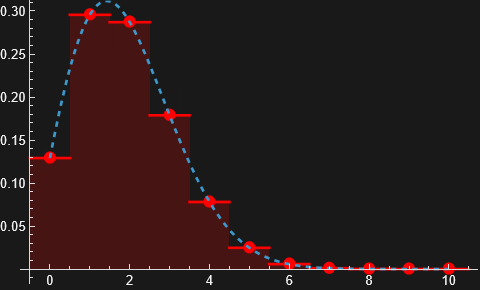
\includegraphics[width=0.7\linewidth]{grafico414}
	\label{fig:grafico414}
\end{figure}

\qed

%%%%%%%%%%%%%%%%%%%%%%%%%%%%%%%%%%%%%%%%%%%%%%%%%%%%%%%%%%%%%%%%%%%%%%%%%%%%%%%%%%%%%%%%%%%%%%%%%%%%%%%%
\section{Problema 4.15}
Show that
\begin{equation}
	Q(N,V,T) = \frac{\left[q(V,T)\right]^N}{N!}
\end{equation}
implies that $q(V,T) = f(T)V$. Do this in both the canonical ensemble and the grand canonical ensemble formalisms.
\resp \textbf{Para el ensamble canónico:} La energía de Helmholtz viene dada por
\begin{equation*}
	F = -kT\ln Q
\end{equation*}
Si en esta ecuación reemplazamos la condición dada por la pregunta, y usamos Stirling para aproximar, llegamos a

\begin{align*}
	F &= -kT\ln\frac{q^N}{N!}\\
	&= -NkT\ln q + kT\ln N!\\
	&= -NkT\ln q + NkT\ln N - NkT\\
	&= -NkT\ln\frac{q}{N} - NkT\\
	&= -NkT\left(\ln\frac{q}{N} + 1\right)
\end{align*}
Ya que sabemos que $F$ debe ser extensivo, se cumplirá que la energía de Helmholtz es una función homogénea en sus  variables $N$ y $V$. Si escalamos ambas por un factor $\alpha$ arbitrario
\begin{align*}
	F(\alpha N, \alpha V, T) &= \alpha F(N, V, T)\\
	-\alpha N kT\left(\ln\frac{q(\alpha V, T)}{\alpha N} + 1\right) &= \alpha\cdot\left[-NkT\left(\ln\frac{q(V,T)}{N}+1\right)\right]\\
	\ln\frac{q(\alpha V, T)}{\alpha N} &= \ln\frac{q(V,T)}{N}\\
	\frac{q(\alpha V, T)}{\alpha N} &= \frac{q(V,T)}{N}\\
	q(\alpha V, T) &= \alpha\, q(V, T)
\end{align*}
Ya que $\alpha$ es arbitrario, $q$ debe ser una función homgénea de grado 1 solo para el volumen $V$. Si fijamos $\alpha = 1/V$,
\begin{align*}
	\frac{1}{V}\,q(V,T) &= q\!\left(\frac{1}{V}\cdot V, T\right) \\
	q(V,T) &= V\cdot q(1,T)
\end{align*}
Ya que $q(1,T)$ solo depende de $T$, definimos $f(T) \equiv q(1,T)$ y obtenemos
\begin{equation}
	q(V,T) = f(T)\,V
\end{equation}
\qed

\textbf{Para el ensamble gran canónico:} La función de partición gran canónica se obtiene sumando todas las funciones $Q(N,V,T)$ sobre todos los $N$:
\begin{align*}
	\Xi &= \sum_{N=0}^\infty \lambda^N Q(N,V,T)
\end{align*}
Reemplazando la ecuación de $Q$,
\begin{align*}
	\Xi &= \sum_{N=0}^\infty \frac{\lambda^N q^N}{N!}\\
	&= e^{\lambda q}
\end{align*}
donde $\lambda = e^{\mu/kT}$ es la fugacidad. El potencial gran canónico es, entonces,
\begin{align*}
	\Omega &= -kT\ln\Xi\\
	&= -kT\lambda q\\
	&= -kT e^{\mu/kT} q(V,T)
\end{align*}
Ya que $\Omega$ también debe ser extensivo en $V$, deberá escalar linealmente con $V$, tal que
\begin{align*}
	\Omega(\alpha V,T) = \alpha\,\Omega(V,T)
\end{align*}
Ya que los factores $e^{\mu/kT}$ y $kT$ son independientes de $V$, tendremos que
\begin{equation*}
	q(\alpha V, T) = \alpha\, q(V, T)
\end{equation*}
que es la misma función que en el caso anterior. Usando el mismo razonamiento,
\begin{equation}
	q(V,T) = f(T)\,V
\end{equation}
\qed

%%%%%%%%%%%%%%%%%%%%%%%%%%%%%%%%%%%%%%%%%%%%%%%%%%%%%%%%%%%%%%%%%%%%%%%%%%%%%%%%%%%%%%%%%%%%%%%%%%%%%%%%
\section{Problema 6.1}
The Morse potential is
\begin{equation}
	U(r) = D_e \left(1 - e^{-\beta(r - r_e)}\right)^2
\end{equation}
Show that $\beta = \nu\sqrt{2\pi^2\mu/D_e}$.
\resp Si realizamos una expansión de Taylor para $U(r)$ alrededor de $r_e$ obtenemos
\begin{equation}
	U(r) \approx \beta ^2 D_e (r-r_e)^2 - \beta ^3 D_e (r-r_e)^3 + \mathcal{O}\left(r-r_e\right)^4
\end{equation}
Por lo que, a primer orden, podemos aproximar el potencial de Morse al de un oscilador armónico,
\begin{equation*}
	U(r) \approx \beta ^2 D_e (r-r_e)^2 ~\Rightarrow~ \frac{1}{2} k (r-r_e)^2
\end{equation*}
\begin{equation}
	\Rightarrow k = 2 D_e \beta^2
\end{equation}
Luego, para un oscilador clásico se cumple que la frecuencia de vibración viene dada por
\begin{align}
	\nu &= \frac{1}{2\pi} \sqrt{\frac{k}{\mu}} \nonumber\\
	\Rightarrow k &= 4\pi^2 \nu^2 \mu
\end{align}
donde $\mu$ es la masa reducida. Igualando ambos resultados y resolviendo para $\beta$,
\begin{align}
	2 D_e \beta^2 &= 4\pi^2 \nu^2 \mu \nonumber\\
	\Rightarrow \beta &= \nu\sqrt{2\pi^2\mu/D_e}
\end{align}
\qed

%%%%%%%%%%%%%%%%%%%%%%%%%%%%%%%%%%%%%%%%%%%%%%%%%%%%%%%%%%%%%%%%%%%%%%%%%%%%%%%%%%%%%%%%%%%%%%%%%%%%%%%%
\section{Problema 6.23}
A more accurate expression for the vibrational energy of a diatomic molecule is
\begin{equation}
	\epsilon_n = \left(n + \frac{1}{2}\right)h\nu - \chi_e \left(n + \frac{1}{2}\right)^2 h\nu
\end{equation}
where $\chi_e$ is called the anharmonicity constant. The additional term here represents the first derivations from strictly harmonic behavior. Treating $\chi_e$ as a small parameter, calculate the anharmonic effect on the various thermodynamic functions at least to first order in $\chi_e$.
\resp Partiendo por la función de partición y reemplazando la energía,
\begin{align*}
	Z &= \sum_{n=0}^\infty e^{-\epsilon_n/kT}\\
	&=\sum_{n=0}^\infty e^{-\left[\left(n + \frac{1}{2}\right)h\nu - \chi_e \left(n + \frac{1}{2}\right)^2 h\nu\right]/kT}\\
	&=\sum_{n=0}^\infty e^{-h\nu/kT \left(n + \frac{1}{2}\right)} e^{h\nu/kT \, \chi_e \left(n + \frac{1}{2}\right)^2}
\end{align*}
Reemplazando $u = h\nu/kT$ llegamos a
\begin{equation}
	Z = \sum_{n=0}^\infty e^{-\left(n + \frac{1}{2}\right) u} e^{\chi_e \left(n + \frac{1}{2}\right)^2 u}
\end{equation}
Ya que $\chi_e$ es pequeño, podemos expandir $Z$ a primer orden y obtener, a través de \texttt{Mathematica},
\begin{align}
	Z &\approx \sum _{n=0}^{\infty } \left(e^{\left(-n-\frac{1}{2}\right) u} + \frac{1}{4} \chi_e u (2 n+1)^2 e^{-\left(n+\frac{1}{2}\right) u} + \mathcal{O}\left(\chi_e ^2\right)\right)\\
	&\approx \frac{3 u \chi_e - 4 + (4 + u \chi_e) \cosh (u)}{16 \sinh^3\left(u/2\right)}
\end{align}
donde, al fijar $\chi_e = 0$, deberíamos recuperar el caso armónico $Z_0$
\begin{equation}
	Z_0 = \frac{1}{2 \sinh(u/2)}
\end{equation}
con lo cual, al restarlo a la expresión no armónica aproximada de $Z$, podemos obtener una idea de la forma de la desviación del caso armónico ideal:
\begin{equation}
	Z \approx Z_0 + \chi_e \, u \frac{3 + \cosh (u)}{16 \sinh^3\left(u/2\right)}
\end{equation}
Y podremos obtener el logaritmo natural de esta cantidad aproximando otra vez para $\chi_e$ pequeño
\begin{align}
	\Rightarrow \ln Z &\approx \ln \left[Z_0 + \chi_e \, u \frac{3 + \cosh (u)}{16 \sinh^3\left(u/2\right)}\right]\nonumber\\
	&\approx \ln Z_0 + \chi_e \, u \frac{3 + \cosh (u)}{16 Z_0 \sinh^3\left(u/2\right)} + \mathcal{O}\left(\chi_e ^2\right)\nonumber\\
	&\approx \ln Z_0 + \chi_e \, u \frac{2 \sinh(u/2)\left(3 + \cosh (u)\right)}{16 \sinh^3\left(u/2\right)}\nonumber\\
	&\approx \ln Z_0 + \chi_e \, u \frac{3 + \cosh (u)}{8 \sinh^2\left(u/2\right)}
\end{align}
A partir de aquí podemos calcular algunas funciones termodinámicas. La energía libre de Helmholtz:
\begin{align}
	F &= -kT\ln Z \nonumber\\
	&\approx F_0 - \chi_e\left[ u kT \frac{3 + \cosh (u)}{8 \sinh^2\left(u/2\right)}\right]
\end{align}
La energía interna (donde consideramos que $\lpd{u}{T} = -u/T$):
\begin{align}
	\pr{E} &= kT^2 \pd{\ln Z}{T}\nonumber\\
	&\approx \pr{E_0} -  \chi_e \left[u k T \frac{3 + \cosh (u)-4 u \coth \left(u/2\right)}{4 (\cosh (u)-1)}\right]
\end{align}
Y la capacidad calórica:
\begin{align}
	C_V &= \pd{\pr{E}}{T}\nonumber\\
	&\approx C_{V0} + \chi_e \left[u^2 k \frac{u (\cosh (u)+2) - 2 \sinh (u)}{4\sinh^4\left(u/2\right)} \right]
\end{align}
Todos estos resultados tienden al caso armónico a medida que $\chi_e$ tiende a cero, mientras que, cuando la temperatura aumenta ($T\rightarrow\infty$ y $u\rightarrow 0$), los efectos no-armónicos crecen.
\qed

%%%%%%%%%%%%%%%%%%%%%%%%%%%%%%%%%%%%%%%%%%%%%%%%%%%%%%%%%%%%%%%%%%%%%%%%%%%%%%%%%%%%%%%%%%%%%%%%%%%%%%%%
\section{Problema 9.1}
Consider the reaction $A \rightleftharpoons 2B$. The canonical ensemble partition function for an ideal binary mixture is
\begin{equation}
	Q(N_A,N_B,V,T) = \frac{q_A^{N_A} q_B^{N_B}}{N_A! N_B!}
\end{equation}
Minimize the Helmholtz free energy with the stoichiometric constraint $2N_A + N_B = \mathrm{constant}$ to show that
\begin{equation}
	\frac{N_B^{*2}}{N_A^{*}} = \frac{q_B^2}{q_A}
\end{equation}
where $N_A^{*}$ and $N_B^{*}$ are the equilibrium numbers of $A$ and $B$. Can you generalize this approach to the reaction $\nu_A A + \nu_B B \rightleftharpoons \nu_C C + \nu_D D$ and derive
\begin{equation}
	\frac{N_C^{\nu_C} N_D^{\nu_D}}{N_A^{\nu_A} N_B^{\nu_B}} = \frac{q_C^{\nu_C} q_D^{\nu_D}}{q_A^{\nu_A} q_B^{\nu_B}}
\end{equation}
\resp La energía libre de Helmholtz puede ser escrita y aproximada utilizando Stirling, tal que
\begin{align}
	F &= -kT\ln Q \nonumber\\
	&= -kT\ln \frac{q_A^{N_A} q_B^{N_B}}{N_A! N_B!} \nonumber\\
	&\approx -kT\left[N_A\ln q_A + N_B\ln q_B - N_A\ln N_A + N_A - N_B\ln N_B + N_B\right] \nonumber\\
	&\approx -kT N_A \left[1 + \ln q_A - \ln N_A\right] - kT N_B \left[1 + \ln q_B - \ln N_B\right]
\end{align}
La \textit{constraint} dada nos dice que
\begin{equation}
	2N_A + N_B = \mathrm{const.}
\end{equation}
O, de otra forma, que por cada $A$ que reacciona, 2 $B$ son creados, por lo que
\begin{equation}
	dN_B = -2 \, dN_A
\end{equation}
Ya que $F$ debe minimizarse, buscaremos que $dF = 0$, tendremos entonces que
\begin{equation*}
	dF = -SdT - pdV + \sum_{j} \mu_j dN_j = 0
\end{equation*}
Asumiendo que trabajamos a $T,V$ constantes $\left(\mu_j \rightarrow \lpd{F}{N_j}\right)$,
\begin{align*}
	dF &= \pd{F}{N_A}dN_A + \pd{F}{N_B}dN_B\\
	&= \pd{F}{N_A}dN_A - 2 \pd{F}{N_B}dN_A\\
	&= \left(\pd{F}{N_A} - 2 \pd{F}{N_B}\right) dN_A = 0
\end{align*}
\begin{equation}
	\Rightarrow \pd{F}{N_A} = 2 \pd{F}{N_B}
\end{equation}
Calculando las derivadas a partir de $F$,
\begin{align*}
	-kT\ln\frac{q_A}{N_A} &= - 2 kT\ln\frac{q_B}{N_B}\\
	-kT\ln\frac{q_A}{N_A} &= - kT\ln\left[\frac{q_B}{N_B}\right]^2
\end{align*}
\begin{align}
	\Rightarrow \frac{q_A}{N^{*}_A} &= \left[\frac{q_B}{N^{*}_B}\right]^2 \nonumber\\
	\Rightarrow \frac{N_B^{*2}}{N_A^{*}} &= \frac{q_B^2}{q_A}
\end{align}
\qed

Luego, para la reacción general $\nu_A A + \nu_B B \rightleftharpoons \nu_C C + \nu_D D$, empezamos por la función de partición para una mezcla ideal de 4 componentes:
\begin{align}
	Q &= \frac{q_A^{N_A}q_B^{N_B}q_C^{N_C}q_D^{N_D}}{N_A!\,N_B!\,N_C!\,N_D!}\\
	\Rightarrow F &\approx -kT \sum_{j} N_j \left[1 + \ln q_j - \ln N_j\right]
\end{align}
Definiendo una variable $\lambda$ tal que $dN_j = \nu_j d\lambda$, donde $j = A,B,C,D$ y $\nu_j$ es tomado positivo para los productos y negativo para los reactantes, tendremos
\begin{equation*}
	dN_A = -\nu_A\,d\lambda, ~~~~~ dN_B = -\nu_B\,d\lambda, ~~~~~ dN_C = +\nu_C\,d\lambda, ~~~~~ dN_D = +\nu_D\,d\lambda
\end{equation*}
Luego, minimizando $F ~\Rightarrow~ dF = 0$, tendremos
\begin{equation*}
	dF = -SdT - pdV + \sum_{j} \mu_j dN_j = 0
\end{equation*}
Asumiendo que trabajamos a $T,V$ constantes,
\begin{align*}
	dF &= \sum_j \mu_j dN_j\\
	&= \left(-\nu_A\mu_A - \nu_B\mu_B + \nu_C\mu_C + \nu_D\mu_D\right)d\lambda = 0
\end{align*}
Ya que $d\lambda$ es arbitario, tendremos que 
\begin{equation}
	-\nu_A\mu_A - \nu_B\mu_B + \nu_C\mu_C + \nu_D\mu_D = 0
\end{equation}
Usando
\begin{equation*}
	\mu_j = \pd{F}{N_j} = -kT \pd{\ln Q}{N_j} = - kT \left(\ln q_j - \ln N_j\right) =  - kT \ln\frac{q_j}{N_j}
\end{equation*}
obtenemos
\begin{align}
	\nu_A\mu_A + \nu_B\mu_B &= \nu_C\mu_C + \nu_D\mu_D \nonumber\\
	-kT \nu_A \pd{\ln Q}{N_A} - kT \nu_B \pd{\ln Q}{N_B} &= - kT \nu_C \pd{\ln Q}{N_C} - kT \nu_D \pd{\ln Q}{N_D} \nonumber\\
	\nu_A\ln\frac{q_A}{N_A} + \nu_B\ln\frac{q_B}{N_B} &= \nu_C\ln\frac{q_C}{N_C} + \nu_D\ln\frac{q_D}{N_D} \nonumber\\
	\ln\left(\frac{q_A}{N_A}\right)^{\nu_A} + \ln\left(\frac{q_B}{N_B}\right)^{\nu_B} &= \ln\left(\frac{q_C}{N_C}\right)^{\nu_C} + \ln\left(\frac{q_D}{N_D}\right)^{\nu_D} \nonumber\\
	\ln\left(\frac{q_A^{\nu_A} q_B^{\nu_B}}{N_A^{\nu_A} N_B^{\nu_B}}\right) &= \ln\left(\frac{q_C^{\nu_C} q_D^{\nu_D}}{N_C^{\nu_C} N_D^{\nu_D}}\right) \nonumber\\
	\Rightarrow \frac{q_A^{\nu_A} q_B^{\nu_B}}{N_A^{\nu_A} N_B^{\nu_B}} &= \frac{q_C^{\nu_C} q_D^{\nu_D}}{N_C^{\nu_C} N_D^{\nu_D}} \nonumber\\
	\Rightarrow \frac{N_C^{\nu_C} N_D^{\nu_D}}{N_A^{\nu_A} N_B^{\nu_B}} &= \frac{q_C^{\nu_C} q_D^{\nu_D}}{q_A^{\nu_A} q_B^{\nu_B}}
\end{align}
\qed

%%%%%%%%%%%%%%%%%%%%%%%%%%%%%%%%%%%%%%%%%%%%%%%%%%%%%%%%%%%%%%%%%%%%%%%%%%%%%%%%%%%%%%%%%%%%%%%%%%%%%%%%









\end{document}